\hypertarget{interfaceBindings}{
\section{Bindings  Interface Reference}
\label{interfaceBindings}\index{Bindings@{Bindings}}
}
Inheritance diagram for Bindings:\begin{figure}[H]
\begin{center}
\leavevmode
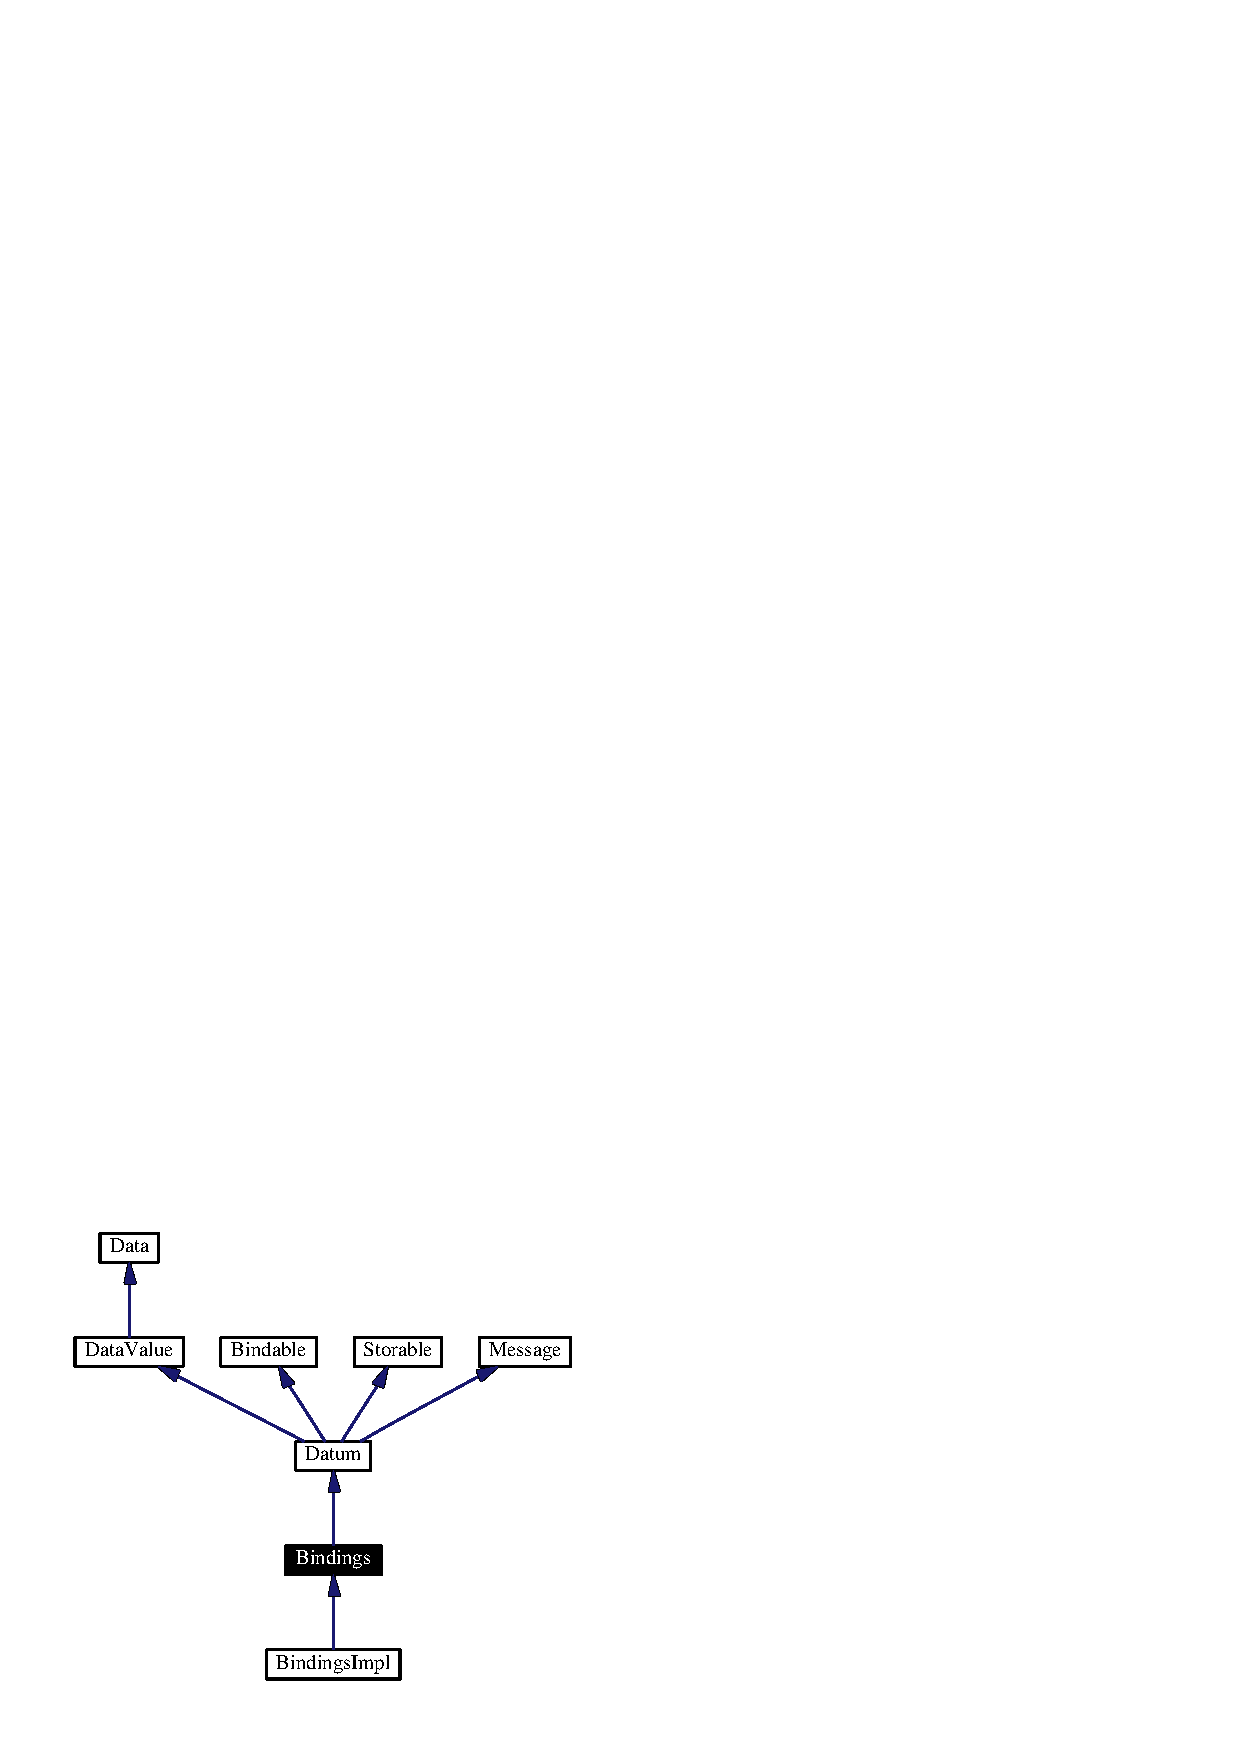
\includegraphics[width=137pt]{interfaceBindings__inherit__graph}
\end{center}
\end{figure}
Collaboration diagram for Bindings:\begin{figure}[H]
\begin{center}
\leavevmode
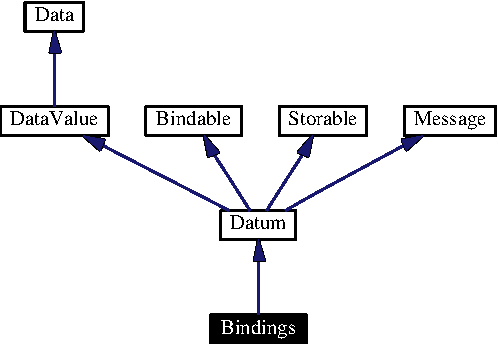
\includegraphics[width=137pt]{interfaceBindings__coll__graph}
\end{center}
\end{figure}
\subsection*{Public Methods}
\begin{CompactItemize}
\item 
Map \hyperlink{interfaceBindings_a0}{map\-Value} ()
\item 
Bindings \hyperlink{interfaceBindings_a1}{binding} (\hyperlink{interfaceToken}{Token} token, \hyperlink{interfaceBindable}{Bindable} bindable)
\item 
\hyperlink{interfaceBindable}{Bindable} \hyperlink{interfaceBindings_a2}{bound} (\hyperlink{interfaceToken}{Token} token) throws \hyperlink{classExceptional}{Exceptional}
\item 
Bindings \hyperlink{interfaceBindings_a3}{overriding} (Bindings bindings)
\item 
Bindings \hyperlink{interfaceBindings_a4}{disjoint\-Union} (Bindings bindings)
\end{CompactItemize}


\subsection{Member Function Documentation}
\hypertarget{interfaceBindings_a1}{
\index{Bindings@{Bindings}!binding@{binding}}
\index{binding@{binding}!Bindings@{Bindings}}
\subsubsection[binding]{\setlength{\rightskip}{0pt plus 5cm}Bindings Bindings::binding (\hyperlink{interfaceToken}{Token} {\em token}, \hyperlink{interfaceBindable}{Bindable} {\em bindable})}}
\label{interfaceBindings_a1}




Reimplemented in \hyperlink{classBindingsImpl_a1}{Bindings\-Impl}.\hypertarget{interfaceBindings_a2}{
\index{Bindings@{Bindings}!bound@{bound}}
\index{bound@{bound}!Bindings@{Bindings}}
\subsubsection[bound]{\setlength{\rightskip}{0pt plus 5cm}\hyperlink{interfaceBindable}{Bindable} Bindings::bound (\hyperlink{interfaceToken}{Token} {\em token})}}
\label{interfaceBindings_a2}




Reimplemented in \hyperlink{classBindingsImpl_a2}{Bindings\-Impl}.\hypertarget{interfaceBindings_a4}{
\index{Bindings@{Bindings}!disjointUnion@{disjointUnion}}
\index{disjointUnion@{disjointUnion}!Bindings@{Bindings}}
\subsubsection[disjointUnion]{\setlength{\rightskip}{0pt plus 5cm}Bindings Bindings::disjoint\-Union (Bindings {\em bindings})}}
\label{interfaceBindings_a4}




Reimplemented in \hyperlink{classBindingsImpl_a4}{Bindings\-Impl}.\hypertarget{interfaceBindings_a0}{
\index{Bindings@{Bindings}!mapValue@{mapValue}}
\index{mapValue@{mapValue}!Bindings@{Bindings}}
\subsubsection[mapValue]{\setlength{\rightskip}{0pt plus 5cm}Map Bindings::map\-Value ()}}
\label{interfaceBindings_a0}




Reimplemented in \hyperlink{classBindingsImpl_a0}{Bindings\-Impl}.

Referenced by Bindings\-Impl::disjoint\-Union(), and Bindings\-Impl::overriding().

\hypertarget{interfaceBindings_a3}{
\index{Bindings@{Bindings}!overriding@{overriding}}
\index{overriding@{overriding}!Bindings@{Bindings}}
\subsubsection[overriding]{\setlength{\rightskip}{0pt plus 5cm}Bindings Bindings::overriding (Bindings {\em bindings})}}
\label{interfaceBindings_a3}




Reimplemented in \hyperlink{classBindingsImpl_a3}{Bindings\-Impl}.

The documentation for this interface was generated from the following file:\begin{CompactItemize}
\item 
\hyperlink{Bindings_8java-source}{Bindings.java}\end{CompactItemize}
